
\subsection{O protocolo OpenFlow}


%
% Openflow
%
\begin{frame}\frametitle{Openflow}

    \begin{itemize}
    \item Openflow é um protocolo que possibilita experimentos e aplicações
          em SDN
    \end{itemize}
    \begin{figure}[h]
        \centering
        
\includegraphics[scale=0.2]{images/openflow}
    \end{figure}
\end{frame}


%
% Openflow
%
\begin{frame}\frametitle{Openflow}

    \begin{itemize}
        \setlength{\itemsep}{.5cm}
    \item \href{http://archive.openflow.org/documents/openflow-wp-latest.pdf}
        {OpenFlow: Enabling Innovation in Campus Networks} publicado em 2008 
    \item Permitiu que pesquisadores criassem experimentos com novos
          protocolos em redes convencionais.
    \end{itemize}

\end{frame}




%
% Openflow
%
\begin{frame}\frametitle{Definição}

    \begin{itemize}
        \setlength{\itemsep}{.5cm}
        \item Interface de programação para o \emph{switch}
        \item Separa de maneira clara os planos de dados e de controle
        \item Permite controlar a forma como um \emph{switch} executa seu 
            encaminhamento de pacotes
        \item Padrão aberto
    \end{itemize}
\end{frame}


%
% Openflow
%
\begin{frame}\frametitle{Componentes}
    Na arquitetura estabelecida pelo protocolo OpenFlow existem dois papéis
    principais.

    \begin{figure}[h]
        \centering
        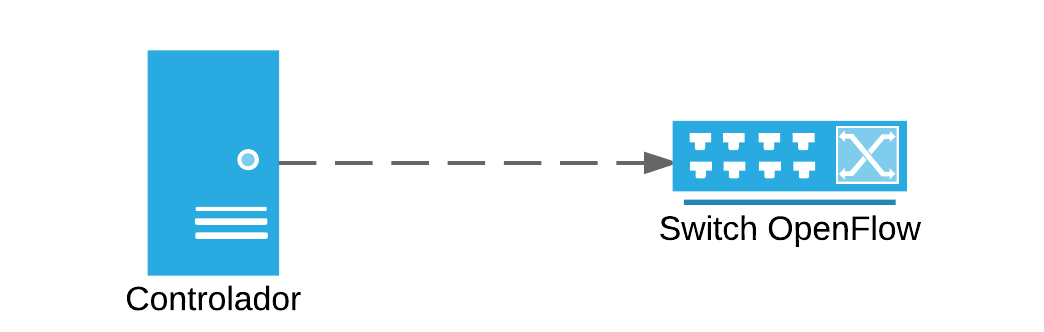
\includegraphics{images/controller-secure-switch}
        \caption{Da esquerda pra direita, plano de controle e plano de dados}
    \end{figure}

\end{frame}


%
% Openflow
%
\begin{frame}\frametitle{Arquitetura OpenFlow}

    \begin{figure}[h!]
        \centering
        \label{fig:switch-arch}
        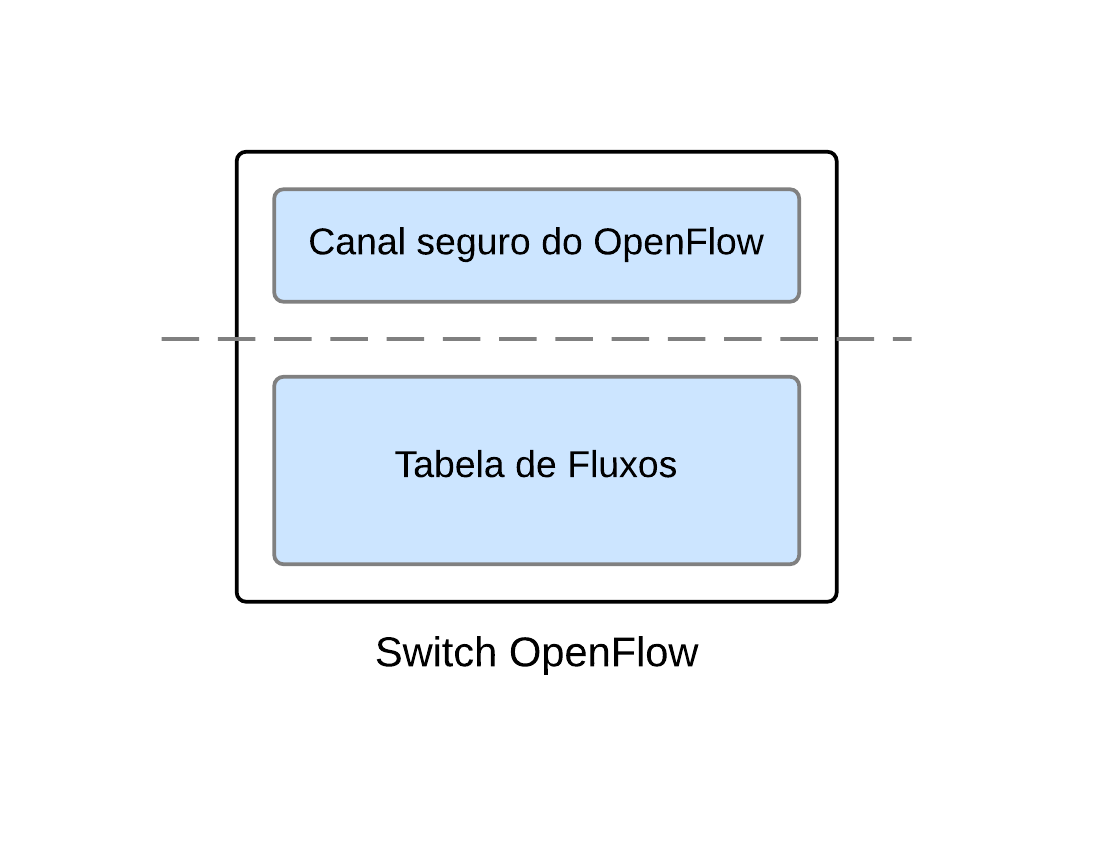
\includegraphics[width=\linewidth]{images/switch-architecture}
        \caption{Arquitetura do comutador OpenFlow}
    \end{figure}

\end{frame}



%
% Switch Archtecture
%
\begin{frame}\frametitle{Tabela de fluxos}
    \begin{table}[h!]
    \small
    \centering
    \begin{tabular}{ | l | l | l | l |}
    \hline
    \textbf{Cabeçalho} & \textbf{Contadores} & \textbf{Ações} &
    \textbf{Prioridade} 
    \\ \hline porta de ingresso=5 & 55635 bytes & \pbox{20cm}{Encaminhar 
    \\ porta=8} 
    & 100 \\ \hline
    \pbox{20cm}{Endereço ip=192.168.1.42 \\ porta=80} & 4032 bytes &
    \pbox{30cm}{Rescrita \\ ip=192.168.1.100} & 500 \\ 
    \hline Protocolo IP=UDP & 100 bytes 
    & Drop & 700 \\ \hline
    \end{tabular}
    \caption{Tabela de fluxos simplificada}
    \label{tbl:flowtable}
\end{table}

\end{frame}

%
% Switch Archtecture
%
\begin{frame}\frametitle{Cabeçalho OpenFlow}

    \begin{itemize}
    \item Um fluxo é identificado pelos seguintes campos do cabeçalho 
          Openflow:
    \end{itemize}
	\begin{figure}[h]\hspace*{-1.2cm}
        \centering
        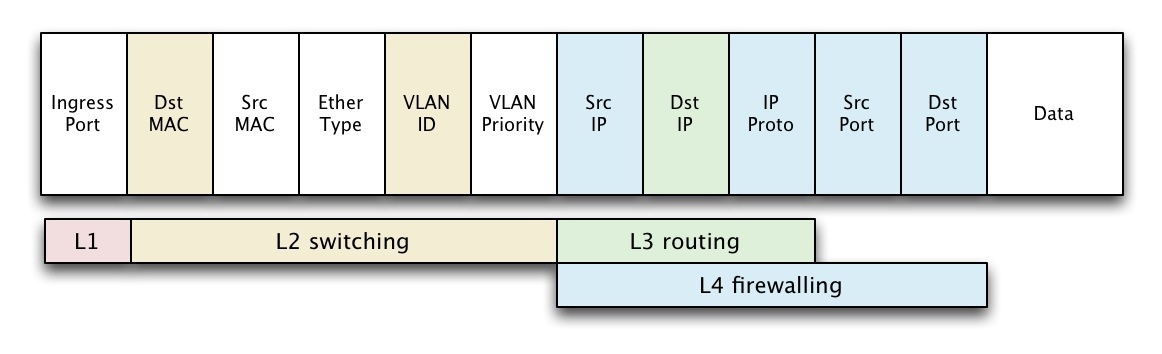
\includegraphics[width=\linewidth]{images/openflow-header}
    \end{figure}
\end{frame}



%
% Actions
%
\begin{frame}\frametitle{Ações}

	\begin{figure}[h]
        \centering
        
\includegraphics[scale=0.5]{images/action.png}
    \end{figure}
    
\end{frame}


%
% Actions
%
\begin{frame}\frametitle{Tipos de ações}

    \begin{columns}[T] % align columns
        \begin{column}{.33\textwidth}

            \begin{itemize}
                \item Forwarding
                \item Drop
                \item Set
                \item strip
                \item Copy-in
                \item Copy-out
                \item Push
                \item Pop
                \item Dec
            \end{itemize}
        \end{column}%
        \hfill%
        \begin{column}{.67\textwidth}
            \begin{figure}[!htb]
                \centering
                
\includegraphics[scale=0.5]{images/action-types}
            \end{figure}
        \end{column}%
    \end{columns}

\end{frame}

%
% Controller
%
\begin{frame}\frametitle{Controlador}

    \begin{itemize}
    \item Controladores Openflow:
          \begin{itemize}
          \item Biblioteca \href{http://opennetworkingfoundation.github.io/libfluid/index.html}{Libfluid}
                para criação de aplicações/controladores em SDN
          \item \href{http://www.noxrepo.org/nox/about-nox/}{Nox Controller}
          \item \href{https://openflow.stanford.edu/display/Beacon/Home}{Beacon}
          \item \href{http://www.noxrepo.org/pox/about-pox/}{Pox Controller}
          \item \href{http://osrg.github.io/ryu/}{Ryu}
          \end{itemize}
    \end{itemize}
\end{frame}
